%-----------------------Homework------------------------------------
%-------------------Arman Shokrollahi---------------------------------
%---------------------Coding Theory-------------------------------

\documentclass[a4 paper]{article}
% Set target color model to RGB
\input{preamble.tex}

\begin{document}
\homework{Práctia \#3}{Mar. 14 al 15 de 2019}{MSc. Fausto M. Lagos S.}{}{Aquí va su nombre}{}

En esta práctica se desarrollarán siete planteamientos cada uno con una valoración de un punto. El objetivo de estas prácticas es afianzar sus conocimientos antes de la Prueba de Evaluación Continua correspondiente, puede utilizar todo el material bibliográfico a su disposición y también preguntar todo lo que considere necesario. Preste atención al margen derecho donde encontrará premios y bonificaciones adicionales.

\vspace{5mm}

\begin{paracol}{2}
\problem{1} Una tienda de campaña con forma de pirámide cuadrangular se construye a partir de una pieza cuadrada de material de 5 mts de lado. En la base de la pirámide, sea $x$ mts la distancia desde el centro a uno de sus lados. \textbf{(a)} Encuentre un modelo matemático que exprese el volumen de la casa de campaña como una función de $x$. \textit{Sugerencia:} La fórmula para el volumen de una pirámide es $V = \frac{1}{3}Bh$, donde $V,\; B$ y $h$ son, respectivamente, las medidas del volumen, el área de la base y la altura. \textbf{b)} Determine el dominio de la función $V(x)$ en el contexto dado. \textbf{c)} Encuentre con aproximación de centésimos de metro, el valor de $x$ para el cual el volumen de la pirámide es máximo. Apoye sus respuentas en la graficadora.
\switchcolumn
\begin{figure}[ht]
    \centering
    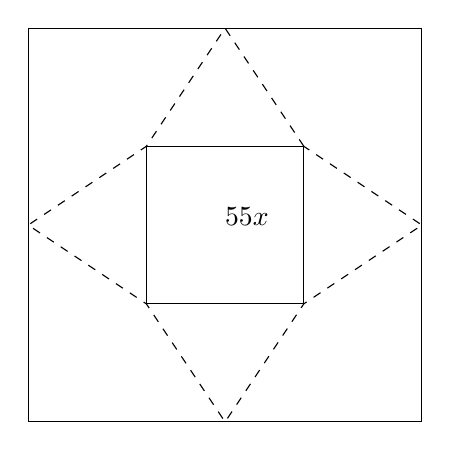
\begin{tikzpicture}
        \draw (-2.5, -2.5) rectangle (2.5, 2.5);
        \draw (-1, -1) rectangle (1, 1);
        \draw[dashed] (1, 1) -- (0, 2.5) -- (-1, 1) -- (-2.5, 0) -- (-1, -1) -- (0, -2.5) -- (1, -1) -- (2.5, 0) -- cycle;
        \dimline[extension start length = .5cm, extension end length = .5cm]{(-2.5, 3)}{(2.5, 3)}{$5$};
        \dimline[extension start length = .5cm, extension end length = .5cm]{(-3, -2.5)}{(-3, 2.5)}{$5$};
        \dimline[extension start length = 0cm, extension end length = 0cm]{(0, 0)}{(1, 0)}{$x$};
    \end{tikzpicture}
\end{figure}
\end{paracol}

\vskip 3mm
\solution{}
\vspace{30mm}

\problem{2} Lea sobre los modelos de proporcionalidad directa e inversa en su libro, sección 1.9 y resuelva: El periodo (tiempo para una oscilación completa) de un péndulo es \textit{directamente proporcional} a la raíz cuadrada de la longitud del péndulo, y un péndulo de 8 ft de longitud tiene un periodo de 2 s. \textbf{(a)} Encuentre un modelo matemático que exprese el periodo de un péndulo como una función de su longitud. \textbf{(b)} Determine el periodo de un péndulo de 2 ft de longitud.

\vskip 3mm
\solution{}
\vspace{30mm}

\problem{3} Sea 
\[f(x) = 
    \begin{cases}
        x, & x < 1 \\
        x^2, & 1 \leq x \leq 9 \\
        27\sqrt{x}, & 9 < x
    \end{cases}
\]
Demuestre que $f$ es inversible y calcule $f^{-1}(x)$.
\vskip 3mm
\solution{}
\vspace{30mm}

\problem{4} \marginnote{\includegraphics[scale = 1]{overleaf}} Trace en la graficadora las gráficas de las dos funciones $F$ y $G$ definidas por
\[
  F(x) = \frac{\sqrt{x + 1}}{\sqrt{x - 4}} \;\;\;\text{ y }\;\;\; G(x) = \sqrt{\frac{x + 1}{x - 4}}
\]
Justifique (analíticamente) por qué las gráficas de $F$ y $G$ no son las mismas y, consecuentemente, las funciones no son iguales.
\vskip 3mm
\solution{}
\vspace{50mm}

\problem{5} Defina las siguientes funciones y determine el dominio de la función resultante \textbf{(a)} $f + g$; \textbf{(b)} $f - g$; \textbf{(c)} $f\cdot g$; \textbf{(d)} $\frac{f}{g}$; \textbf{(e)} $\frac{g}{f}$. para 
\[
  f(x) = \frac{1}{x + 1};\;\;\; g(x) = \frac{x}{x - 2}
\]
\vskip 3mm
\solution{}
\vspace{30mm}


\problem{6} \textbf{(a)} Defina a trozos la función dada en los intervalos indicados. \textbf{(b)} Establezca graficamente si la función es par, impar o de ninguno de estos dos tipos. \textbf{(c)} Confirme analíticamente la respuesta del inciso (b).
\[
    f(x) = \frac{|x|}{x}; \;\; (-\infty, 0), (0, \infty)
\]

\vskip 3mm
\solution{}
\vspace{30mm}

\problem{7} ¿Es conmutativa la composición de dos funciones? Es decir, si $f$ y $g$ son dos funciones cualesquiera, ¿son iguales $(f\circ g)(x)$? y $(g\circ f)(x)$? Justifique su respuesta proporcionando un ejemplo.
\vskip 3mm
\solution{}
\vspace{30mm}

\problem{8} \todo[color = cyan!65!gray]{\small Si resuelve este problema su solución será publicada en la cartelera de matemáticas} The interior bisector of $\angle B$, and the exterior bisector of $\angle C$ of $\triangle ABC$ meet at $D$. Through $D$, a line parallel to $\overline{CB}$ meet $\overline{AC}$ at $L$ and $\overline{AB}$ at $M$. if the measures of legs $\overline{LC}$ and $\overline{MB}$ of trapezoid $CLMB$ are 5 and 7, respectively, find the measure of base $\overline{LM}$. Prove your result.

\textbf{Challenge} Find $\overline{LM}$ if $\triangle ABC$ is equilateral.
\begin{figure}[ht]
    \centering
    \begin{tikzpicture}
        \coordinate[label = above:{$A$}] (A) at (2, 3);
        \coordinate[label = right:{$B$}] (B) at (5, 0);
        \coordinate[label = below:{$C$}] (C) at (0, 0);
        \coordinate[label = left:{$D$}] (D) at (-2, 2);
        \coordinate (f) at (5, 2);
        
        \draw[name path = AB] (A) -- (B);
        \draw[name path = AC] (A) -- (C);
        \draw (C) -- (D);
        \draw (C) -- (B);
        \draw[name path = DB] (D) -- (B);
        
        \path[name intersections = {of = DB and AC}];
        \coordinate[label = below:{$E$}] (E) at (intersection-1);
        
        \path[name path = Df] (D) -- (f);
        \path[name intersections = {of = Df and AB}];
        \coordinate[label = right:{$M$}] (L) at (intersection-1);
        \draw (D) -- (intersection-1);
        \path[name intersections = {of = Df and AC}];
        \coordinate[label = above left:{$L$}] (L) at (intersection-1);
    \end{tikzpicture}
\end{figure}
\end{document}
